\usetikzlibrary{positioning}
% \usetikzlibrary{arrows.meta}
\usetikzlibrary{bending}
\usetikzlibrary{backgrounds}
\definecolor{red}{HTML}{8A3F3A}
\definecolor{yellow}{HTML}{E0BB3C}
\definecolor{blue}{HTML}{4569E0}
\definecolor{green}{HTML}{17E561}
\definecolor{other}{HTML}{6A939E}

% DTU Colors
\definecolor{dtu-corporate-red}{HTML}{990000}
\definecolor{dtu-white}{HTML}{ffffff}
\definecolor{dtu-black}{HTML}{000000}
\definecolor{dtu-blue}{HTML}{2F3EEA}
\definecolor{dtu-bright-green}{HTML}{1FD082}
\definecolor{dtu-navy-blue}{HTML}{030F4F}
\definecolor{dtu-yellow}{HTML}{F6D04D}
\definecolor{dtu-orange}{HTML}{FC7634}
\definecolor{dtu-pink}{HTML}{F7BBB1}
\definecolor{dtu-grey}{HTML}{DADADA}
\definecolor{dtu-red}{HTML}{E83F48}
\definecolor{dtu-green}{HTML}{008835}
\definecolor{dtu-purple}{HTML}{79238E}


\newlength{\basisc}
\setlength{\basisc}{0.5cm}

\centering
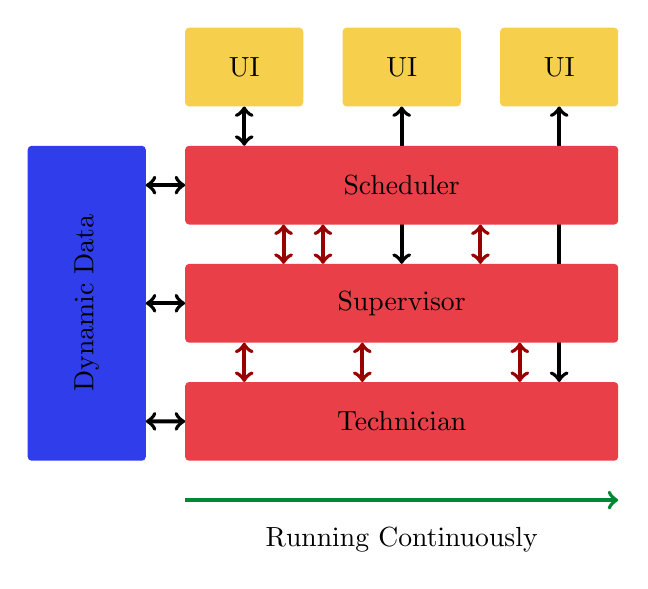
\begin{tikzpicture}[line width=0.0\basisc]
    \draw (4.0\basisc,4.0\basisc) 
		node[rotate=90, minimum height=3\basisc,fill=dtu-blue,minimum width=8\basisc,rounded corners=0.1\basisc] 
			(Dynamic Data) {Dynamic Data};

			

    \draw (8.0\basisc,10.0\basisc) 
		node[minimum height=2\basisc,fill=dtu-yellow,minimum width=3\basisc,rounded corners=0.1\basisc] 
			(UserInterface1) {UI};
    \draw (12.0\basisc,10.0\basisc) 
		node[minimum height=2\basisc,fill=dtu-yellow,minimum width=3\basisc,rounded corners=0.1\basisc] 
			(UserInterface2) {UI};
    \draw (16.0\basisc,10.0\basisc) 
		node[minimum height=2\basisc,fill=dtu-yellow,minimum width=3\basisc,rounded corners=0.1\basisc] 
			(UserInterface3) {UI};
    \draw (12.0\basisc,7.0\basisc) 
		node[minimum height=2\basisc,fill=dtu-red,minimum width=11\basisc,rounded corners=0.1\basisc] 
			(Scheduler) {Scheduler};
    \draw (12.0\basisc,4.0\basisc) 
		node[minimum height=2\basisc,fill=dtu-red,minimum width=11\basisc,rounded corners=0.1\basisc] 
			(Supervisor) {Supervisor};
    \draw (12.0\basisc,1.0\basisc) 
		node[minimum height=2\basisc,fill=dtu-red,minimum width=11\basisc,rounded corners=0.1\basisc] 
			(Technician) {Technician};


	\begin{pgfonlayer}{background}
		\draw[<->, thick, line width=0.1\basisc] (UserInterface1) to[out=-90, in=90,looseness=1.0] ++(0\basisc,-2.0\basisc)(Scheduler);
		\draw[<->, thick, line width=0.1\basisc] (UserInterface2) to[out=-90, in=90,looseness=1.0] (Supervisor);
		\draw[<->, thick, line width=0.1\basisc] (UserInterface3) to[out=-90, in=90,looseness=1.0] ++(0\basisc,-8.0\basisc)(Technician);

	\end{pgfonlayer}

	\draw[->, line width=0.1\basisc,color=dtu-green] (6.5\basisc, -1\basisc) -- (17.5\basisc, -1\basisc);
	\draw (12.0\basisc, -2.0\basisc) node {Running Continuously};

	\draw[<->, thick, line width=0.1\basisc, color=dtu-corporate-red] (Scheduler)++(-3\basisc, -1.0\basisc) to[out=-90, in=90,looseness=1.0]  ++(0\basisc, -1.0\basisc)(Supervisor);
	\draw[<->, thick, line width=0.1\basisc, color=dtu-corporate-red] (Scheduler)++(-2\basisc, -1.0\basisc) to[out=-90, in=90,looseness=1.0]  ++(0\basisc, -1.0\basisc)(Supervisor);
	\draw[<->, thick, line width=0.1\basisc, color=dtu-corporate-red] (Scheduler)++(2\basisc, -1.0\basisc) to[out=-90, in=90,looseness=1.0]  ++(0\basisc, -1.0\basisc)(Supervisor);

	\draw[<->, thick, line width=0.1\basisc, color=dtu-corporate-red] (Supervisor)++(-4\basisc, -1.0\basisc) to[out=-90, in=90,looseness=1.0] ++(0\basisc, -1.0\basisc)(Technician);
	\draw[<->, thick, line width=0.1\basisc, color=dtu-corporate-red] (Supervisor)++(-1\basisc, -1.0\basisc) to[out=-90, in=90,looseness=1.0] ++(0\basisc, -1.0\basisc)(Technician);
	\draw[<->, thick, line width=0.1\basisc, color=dtu-corporate-red] (Supervisor)++(3\basisc, -1.0\basisc) to[out=-90, in=90,looseness=1.0] ++(0\basisc, -1.0\basisc)(Technician);

	\draw[<->, thick, line width=0.1\basisc] (Dynamic Data.south) ++(0\basisc,3.0\basisc) to[out=0, in=180,looseness=1.0] (Scheduler);
	\draw[<->, thick, line width=0.1\basisc] (Dynamic Data.south) to[out=0, in=180,looseness=1.0] (Supervisor);
	\draw[<->, thick, line width=0.1\basisc] (Dynamic Data.south) ++(0\basisc,-3.0\basisc) to[out=0, in=180,looseness=1.0] (Technician.west);

	% \draw[<->, thick, line width=0.1\basisc] (Scheduler) -- (UserInterface);
\end{tikzpicture}
